\documentclass[11pt,a4paper]{article}
\usepackage[utf8]{inputenc}
\usepackage[T1]{fontenc}
\usepackage{lmodern}
\usepackage[a4paper,margin=2.4cm]{geometry}
\usepackage{setspace,microtype,graphicx,booktabs,tabularx,array,longtable,enumitem,hyperref,xcolor,float,caption}
\usepackage{tikz}
\usetikzlibrary{arrows.meta,positioning,shapes.geometric,calc}
\usepackage[backend=biber,style=authoryear,sorting=nyt,maxcitenames=2,maxbibnames=99]{biblatex}
\addbibresource{references.bib}
\hypersetup{colorlinks=true,linkcolor=blue!50!black,citecolor=blue!50!black,urlcolor=blue!60!black,pdftitle={Task 2 - Technical Report: Responsible AI Assessment of BrainWaveNet},pdfauthor={Levi Pedro Tejedor Rico}}
\setstretch{1.12}
\setlist[itemize]{leftmargin=*,itemsep=3pt,topsep=3pt}
\setlist[enumerate]{leftmargin=*,itemsep=3pt,topsep=3pt}
\newcolumntype{Y}{>{\raggedright\arraybackslash}X}
\newcommand{\ASD}{\textsc{asd}}
\newcommand{\PBG}{\textsc{pbg}}

\title{\textbf{Task 2: Technical Report}\\
\large Responsible AI Assessment of BrainWaveNet for Autism Spectrum Disorder Classification}
\author{Levi Pedro Tejedor Rico\\Student ID: 4506001}
\date{Module: CSI\_7\_DEL -- Deep Learning}

\begin{document}
\maketitle

\begin{abstract}
This report evaluates BrainWaveNet, a wavelet-based Transformer that classifies autism spectrum disorder (ASD) and typically developing participants using resting-state functional MRI. The assessment combines the SUM values (Respect, Connect, Protect and Care), FAST principles (Fairness, Accountability, Sustainability and Transparency), and a process-based governance (PBG) approach across the AI lifecycle. BrainWaveNet is a promising research prototype evaluated on a subset of ABIDE-I, but its reported classification performance, lack of external clinical validation and limited evidence of stakeholder participation do not support clinical diagnostic use. The analysis identifies risks associated with multi-site data, sample selection, subgroup uncertainty, test-set governance, interpretability and the absence of a clinical monitoring system. It proposes governance gates, accountable roles, social impact assessment checkpoints and corrective controls. The recommendation is to retain the model for research until independent validation, autistic community participation and clinical safety governance have been demonstrated.
\end{abstract}

\tableofcontents
\newpage

\section{Introduction}
Artificial intelligence (AI) is increasingly investigated in healthcare because it may support analysis of complex clinical and biomedical data. However, technical performance alone is insufficient to justify deployment: systems can reproduce structural inequalities, obscure responsibility or create harms when used outside the conditions in which they were evaluated. Health AI therefore requires lifecycle governance, meaningful human oversight and evidence that the intended application benefits patients and communities \parencite{who2021,rajkomar2018,leslie2019}.

This report examines BrainWaveNet, a deep-learning research model for classifying ASD and typically developing (TD) participants from resting-state functional magnetic resonance imaging (rs-fMRI). The coursework objectives are to describe the project and its evidence base; assess it using SUM and FAST; examine each lifecycle phase; and propose a PBG framework that translates ethical commitments into controls, responsibilities and release decisions. The report uses the published BrainWaveNet study, ABIDE-I documentation and implementation repository as primary project evidence, supplemented by literature on fairness, accountability, neuroimaging reproducibility and healthcare AI.

The scope is deliberately bounded. BrainWaveNet is treated as a research prototype, not as a clinically deployed diagnostic product. Consequently, the report distinguishes documented properties from missing evidence and foreseeable risks. A missing control in a research paper is not automatically proof of misconduct or an existing patient harm; it is a gap that must be resolved before a higher-risk use can be considered.

\section{AI Project Background}
\subsection{Clinical and data context}
Autism is a heterogeneous neurodevelopmental condition. Clinical identification is based on developmental history and behavioural assessment rather than a single neuroimaging measurement. Machine learning research has explored whether brain-imaging patterns can contribute to understanding group-level differences, but group-level statistical findings do not necessarily translate into reliable individual diagnosis. Large-scale functional connectivity work has identified reproducible alterations while also highlighting the complexity and overlap of individual patterns \parencite{holiga2019}.

The Autism Brain Imaging Data Exchange (ABIDE-I) is a multi-site research resource that shares structural and resting-state MRI data with phenotypic information. Its initial release included 1,112 participants from 17 sites: 539 participants with ASD and 573 TD controls, aged approximately 7--64 years \parencite{dimartino2014,abidewebsite}. The breadth of sites improves research opportunities but introduces variation in scanners, acquisition protocols, recruitment and participant characteristics. Harmonisation and site-aware evaluation are therefore important; neuroimaging studies have shown that site effects can confound machine-learning results \parencite{abraham2017,abideharmonization2022}.

\subsection{BrainWaveNet method}
\textcite{jeong2024} propose BrainWaveNet to learn spatiotemporal information from rs-fMRI in the frequency domain. The method applies a complex Morlet continuous wavelet transform (CWT) to blood-oxygen-level-dependent time series. It processes real and imaginary coefficients using residual convolutional blocks, frequency token encoding and temporal Transformer encoders, then uses spatial Transformer attention and cross-attention to learn relationships between regions of interest (ROIs). The final representation is used for binary ASD/TD classification.

The authors report using CPAC-preprocessed data, a 0.01--0.1 Hz band-pass filter, no global signal regression, the Craddock 200 atlas and 78 time points per participant. CWT features are represented across five frequency sub-bands, with sampling frequency adjusted for site-specific repetition time. Of the original ABIDE-I cohort, 897 participants remained after quality control: 414 ASD and 483 TD. The reported experimental protocol uses a 7:2:1 training, validation and test split and five-fold cross-validation; model selection is based on validation AUC \parencite{jeong2024}.

\subsection{Reported results and evidential limits}
BrainWaveNet achieved a reported AUC of 0.7388, accuracy of 67.55\%, sensitivity of 66.49\% and specificity of 68.35\% (means across reported folds; standard deviations were 0.02, 2.03, 9.17 and 9.80 respectively) \parencite{jeong2024}. It achieved the highest AUC, accuracy and sensitivity among the comparison methods reported in the paper, but not the highest specificity. These are research classification results, not evidence of clinical utility, calibrated individual risk or improved patient outcomes. The study does not establish prospective performance in a clinical pathway or external validation on an independently collected cohort.

The accompanying public repository improves inspectability, but a code release does not by itself guarantee reproducibility. The repository's displayed results contain small discrepancies from some values in the paper, and the implementation should be reconciled and executed from a documented clean environment before results are treated as independently replicated \parencite{brainwavenetcode}. The model's ROI analysis is also exploratory: selected regions are not automatically causal biomarkers or explanations that clinicians and autistic people can safely interpret.

\section{Responsible AI Assessment}
\subsection{Assessment method}
The analysis applies the SUM values and FAST principles described by \textcite{leslie2019}. It draws on the broader view that sources of harm can arise at every stage of machine-learning development, from problem definition and data collection to deployment \parencite{suresh2021}. Each judgement is evidence-based: where the paper does not report a control, the report records an evidence gap rather than assuming the control is absent in every researcher's practice.

\subsection{SUM values}
\begin{table}[H]
\centering
\caption{SUM assessment of BrainWaveNet.}
\label{tab:sum}
\small
\begin{tabularx}{\textwidth}{p{2.2cm}Y Y}
\toprule
\textbf{Value} & \textbf{Evidence and concern} & \textbf{Required improvement}\\
\midrule
Respect & Autistic participants are included in ABIDE-I, but the BrainWaveNet paper does not report autistic co-design or participation in setting research goals, interpreting results or governing future use. Data representation is not equivalent to agency. & Establish paid and accessible autistic advisory roles with influence over purpose, communication, evaluation and release. Use respectful, non-deficit language and explain limits of brain-based classification.\\
Connect & ABIDE-I is an international collaboration across 17 sites. However, the paper does not document engagement with autistic people, families, clinicians or service organisations. & Map affected stakeholders and co-design the intended use with autistic people and clinical professionals. Record how consultation changes project decisions.\\
Protect & The model is not shown to make autonomous decisions, and ABIDE data were shared under research governance. Nevertheless, neuroimaging and linked phenotypes are sensitive; false results, inappropriate linkage and future misuse are foreseeable. & Apply data minimisation, access controls, secure storage, retention rules and incident response. Prohibit standalone diagnosis and require clinical oversight for any authorised pilot.\\
Care & The research may contribute to understanding, but no evidence shows improved diagnostic experience, reduced waiting times or better outcomes. Reported sensitivity and specificity leave substantial classification error. & Define a patient-relevant benefit and evaluate it prospectively. Never condition access to assessment or support on a model prediction.\\
\bottomrule
\end{tabularx}
\end{table}

Respect is especially important because ASD labels can affect identity, access to services and how people are treated. A model should not imply that an individual can be understood through a scan or that a statistical group difference defines what autism means. Participatory research guidance supports involving autistic people throughout research design and delivery, rather than consulting them only after technical decisions have been made \parencite{albacete2024}. Protect and Care also require proportionate communication: sensitivity and specificity around two-thirds are not adequate grounds for presenting the output as a diagnosis.

\subsection{FAST principles}
\begin{table}[H]
\centering
\caption{FAST assessment of BrainWaveNet.}
\label{tab:fast}
\small
\begin{tabularx}{\textwidth}{p{2.2cm}Y Y}
\toprule
\textbf{Principle} & \textbf{Evidence and concern} & \textbf{Required improvement}\\
\midrule
Fairness & The study reports aggregate performance, not results by age, sex, site or clinical subgroup. Multi-site scanner and recruitment differences may act as confounders; quality-control exclusions may alter the sample. & Publish inclusion/exclusion analyses and subgroup metrics with uncertainty. Conduct site-held-out and external validation, and assess calibration and error rates across relevant groups.\\
Accountability & Authors, paper and code are identifiable, but there is no clinical owner, complaint route, incident process or authority for approving/withdrawing a deployed product. The repository evaluates test metrics during training, creating a test-set peeking risk, although this alone does not prove leakage. & Assign named owners, maintain decision logs and audit trails, lock the test set, and define appeal, incident, pause and withdrawal procedures.\\
Sustainability & Energy, hardware utilisation, carbon footprint, MRI access costs and long-term maintenance are not reported. MRI infrastructure is expensive and unevenly available. & Measure training/inference resources and total workflow costs. Compare expected benefit with MRI burden and less resource-intensive alternatives.\\
Transparency & The paper describes the architecture and evaluation, and code is public. However, code-paper metric discrepancies, incomplete reproducibility information and exploratory ROI rankings limit interpretation. & Publish a model card, dataset factsheet, versioned environment, preprocessing and split scripts, uncertainty statements and plain-language limitations.\\
\bottomrule
\end{tabularx}
\end{table}

Fairness cannot be inferred from a near-balanced ASD/TD label distribution. Bias can enter through recruitment, measurement, missingness, labels and the choice of outcome; it may also persist when aggregate performance appears acceptable \parencite{mehrabi2021,suresh2021}. In healthcare, apparently neutral prediction targets can reproduce inequity when they stand in for unequal access or need, as demonstrated by research on population-health algorithms \parencite{obermeyer2019}. Although that study concerns a different clinical algorithm, it illustrates why the target, data-generating process and downstream consequences must be examined rather than relying on model accuracy alone. Health AI fairness requires explicit attention to equity and the clinical context \parencite{rajkomar2018}.

Accountability should extend beyond model developers. An end-to-end audit framework can make responsibility traceable through design, development and deployment decisions \parencite{raji2020}. Transparency also requires more than publishing source code: model cards provide a structured way to document intended use, evaluation conditions, limitations and subgroup performance \parencite{mitchell2019}. For BrainWaveNet, these artefacts should make clear that the current evidence supports research exploration only.

\subsection{End-to-end lifecycle examination}
\subsubsection{1. Problem formulation}
The technical question is whether rs-fMRI features can distinguish labelled ASD and TD participants. The paper does not establish that the classifier solves a clinical problem identified by autistic people or clinicians, nor does it define a target user, clinical workflow or patient-relevant outcome. This creates a framing risk: a binary dataset label may be mistaken for a complete representation of autism. Before further development, the team should conduct an initial social impact assessment (SIA), define intended and prohibited uses, document the benefit hypothesis and consult autistic stakeholders. The project should be stopped or reframed if no credible benefit can be identified.

\subsubsection{2. Data extraction and acquisition}
ABIDE-I combines data from 17 sites, but the BrainWaveNet analysis retains 897 of 1,112 participants after quality control. The retained sample is approximately balanced by diagnosis, yet this does not demonstrate representation across age, sex, IQ, site or clinical presentation. Phenotypic data completeness varies. Site effects are a recognised challenge in multi-site neuroimaging and can affect reproducibility \parencite{abraham2017,abideharmonization2022}. A dataset factsheet should record provenance, permissions, recruitment context, missingness, quality-control criteria and demographic composition. The team should compare included and excluded participants and avoid assuming that research data permissions automatically authorise clinical use.

\subsubsection{3. Data preprocessing}
The reported pipeline includes CPAC, band-pass filtering, atlas parcellation, fixed-length cropping and CWT. Such transformations may influence which signals are retained and may interact with site and participant differences. The report does not provide a full subgroup analysis of quality-control exclusions or establish that site-related variation has been eliminated. Redevelopment should version every preprocessing step, publish parameter settings, log exclusions, quantify head-motion and missingness effects, and test alternative preprocessing choices. Any harmonisation must be fitted without leaking information from held-out test data.

\subsubsection{4. Modelling, testing and validation}
BrainWaveNet's architecture is technically motivated by frequency-domain and spatiotemporal learning. Nevertheless, AUC 0.7388 and accuracy 67.55\% indicate moderate discrimination rather than a clinically decisive test. Sensitivity and specificity are both around 66--68\%, and their reported variability is notable. No independent external clinical validation or subgroup performance analysis is reported. The repository's repeated test-metric evaluation during training should be reviewed to ensure the test set did not influence decisions. A revised protocol should lock the test set, pre-register thresholds and analyses, use nested or otherwise leakage-safe validation, report confidence intervals and calibration, and test on an independent site or cohort. Neuroimaging performance can be sensitive to site effects and sample composition; harmonisation and validation must therefore be explicitly evaluated \parencite{abraham2017,abideharmonization2022}. The ROI ranking should be tested for stability across folds and cohorts and not described as causal explanation.

\subsubsection{5. Deploy, monitor and release}
The available evidence demonstrates publication and code release, not routine clinical deployment. No clinical safety case, regulatory assessment, prospective trial, workflow integration, user training or post-release monitoring is documented. This is a critical boundary: the model should not be used to diagnose individuals, determine eligibility for support or replace clinical judgement. Any future pilot would require institutional and regulatory review, defined human oversight, clear communication of uncertainty, complaint and adverse-event routes, drift monitoring and a rollback plan. WHO guidance emphasises human autonomy, safety, transparency, accountability and inclusiveness in health AI \parencite{who2021}. Good machine-learning practice for medical devices similarly emphasises lifecycle controls and the performance of the human-AI team \parencite{gmlp2021}. Human expertise should remain central; AI should be assessed as part of a care process, not as a stand-alone substitute for it \parencite{topol2019}.

\subsection{Process-Based Governance framework}
PBG translates principles into operational gates. The proposed governance structure is a redevelopment plan; it does not imply that BrainWaveNet currently has these arrangements. A multidisciplinary board should include a project owner, clinical lead, data/ML lead, data protection and security specialist, independent ethics/fairness reviewer, and autistic community representatives. The community representatives should be resourced and able to influence decisions, not merely endorse a predetermined system.

\begin{figure}[H]
\centering
\resizebox{\textwidth}{!}{%
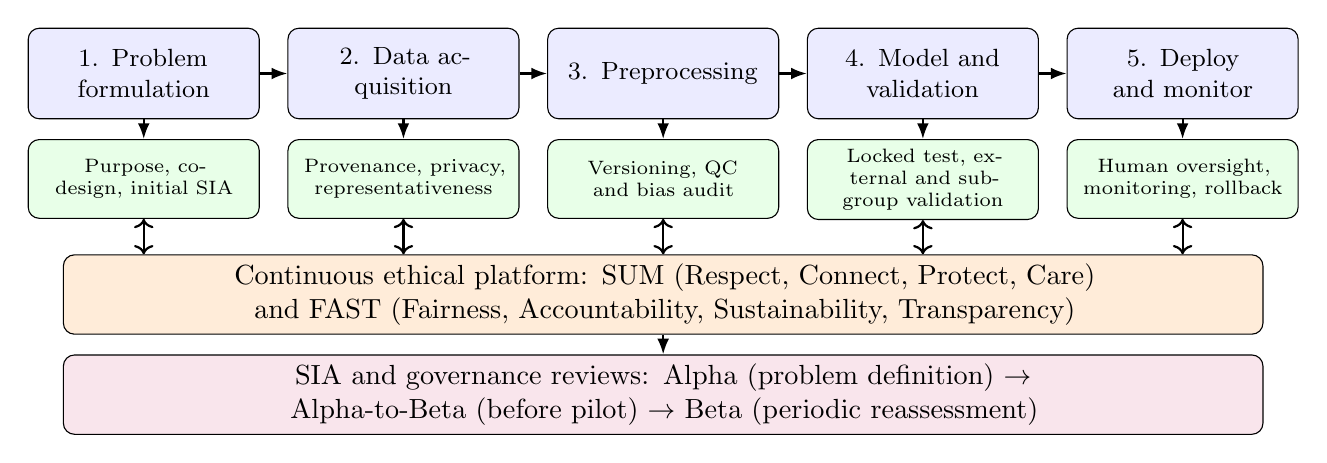
\begin{tikzpicture}[phase/.style={draw,rounded corners,fill=blue!8,text width=2.7cm,minimum height=1.15cm,align=center,font=\small},
ctrl/.style={draw,rounded corners,fill=green!9,text width=2.7cm,minimum height=1.0cm,align=center,font=\scriptsize},
arr/.style={-{Latex[length=2mm]},thick}]
\node[phase] (a) {1. Problem formulation};
\node[phase,right=0.35cm of a] (b) {2. Data acquisition};
\node[phase,right=0.35cm of b] (c) {3. Preprocessing};
\node[phase,right=0.35cm of c] (d) {4. Model and validation};
\node[phase,right=0.35cm of d] (e) {5. Deploy and monitor};
\draw[arr] (a)--(b);\draw[arr] (b)--(c);\draw[arr] (c)--(d);\draw[arr] (d)--(e);
\node[ctrl,below=0.25cm of a] (ca) {Purpose, co-design, initial SIA};
\node[ctrl,below=0.25cm of b] (cb) {Provenance, privacy, representativeness};
\node[ctrl,below=0.25cm of c] (cc) {Versioning, QC and bias audit};
\node[ctrl,below=0.25cm of d] (cd) {Locked test, external and subgroup validation};
\node[ctrl,below=0.25cm of e] (ce) {Human oversight, monitoring, rollback};
\draw[arr] (a)--(ca);\draw[arr] (b)--(cb);\draw[arr] (c)--(cc);\draw[arr] (d)--(cd);\draw[arr] (e)--(ce);
\node[draw,rounded corners,fill=orange!15,align=center,text width=15cm,below=0.45cm of cc] (v) {Continuous ethical platform: SUM (Respect, Connect, Protect, Care) and FAST (Fairness, Accountability, Sustainability, Transparency)};
\foreach \n in {ca,cb,cc,cd,ce} {\draw[<->,thick] (\n.south)--(v.north -| \n.south);}
\node[draw,rounded corners,fill=purple!10,align=center,text width=15cm,below=0.25cm of v] (s) {SIA and governance reviews: Alpha (problem definition) $\rightarrow$ Alpha-to-Beta (before pilot) $\rightarrow$ Beta (periodic reassessment)};
\draw[arr] (v)--(s);
\end{tikzpicture}}
\caption{Proposed process-based governance landscape for BrainWaveNet redevelopment.}
\label{fig:pbg}
\end{figure}

The governance gates should require:
\begin{enumerate}
\item \textbf{Alpha -- problem definition:} initial SIA, intended-use statement, stakeholder map, benefit hypothesis, prohibited uses and initial risk register. Approval is required before data work proceeds.
\item \textbf{Data and preprocessing gate:} provenance and permission records, privacy review, dataset factsheet, inclusion/exclusion analysis, versioned pipeline and bias assessment.
\item \textbf{Model validation gate:} model card, locked test protocol, independent/site-held-out validation, subgroup results, calibration, confidence intervals, error analysis and explanation-stability tests.
\item \textbf{Alpha-to-Beta -- pre-pilot:} updated SIA after technical development, stakeholder consultation, documented changes and public-facing summary. No pilot proceeds without independent clinical, ethical and institutional approval.
\item \textbf{Beta -- reassessment:} periodic review of real-world effects, drift, complaints, adverse events, subgroup performance and changes in context. The governance board must be able to pause, roll back or withdraw the system.
\end{enumerate}
These checkpoints make ethical review continuous rather than a one-off approval. They also complement technical audit and monitoring; they do not replace them \parencite{leslie2019,raji2020}.

\subsection{Priority corrective actions}
The most important corrective actions are: (1) obtain meaningful autistic community participation before deciding whether the intended use is acceptable; (2) document data provenance and quantify selection and subgroup effects; (3) lock the test set and complete independent, site-aware and external validation; (4) publish reproducibility artefacts and a model card; (5) establish accountable clinical, ethical, privacy and security roles; and (6) prohibit clinical use until a safety case, regulatory review, human oversight and monitoring plan are approved. These actions address the central risks without overstating what the current research has demonstrated.

\section{Conclusion}
BrainWaveNet demonstrates a technically interesting approach to learning frequency-based spatiotemporal features from rs-fMRI, and its ABIDE-I results justify further research. However, reported performance is moderate, subgroup fairness is not established, external clinical validation is absent, and the paper does not demonstrate autistic co-design or operational deployment governance. The evidence therefore supports a research-only classification prototype, not a diagnostic product.

A responsible redevelopment should embed SUM and FAST throughout the lifecycle through a PBG framework with named owners, documented evidence and Alpha, Alpha-to-Beta and Beta SIA checkpoints. Progression should depend on meaningful participation by autistic people, transparent and reproducible data/model practices, independent validation across sites and relevant subgroups, and a clinical safety and monitoring system. Until these conditions are met, BrainWaveNet should not influence diagnosis, access to services or treatment decisions.

\printbibliography[heading=bibintoc,title={References}]
\end{document}
